\chapter{Experimenton and Results}

\section{Introduction}
With the configuration described in the previous section we can now start to experiment with the robotic platform to do certain navigation tasks. In this part we propose 2 experiments that show that the \ac{RADAR} can be an alternative or support to the \ac{LiDAR} as an obstacle detector for indoor navigation.

\section {Experiment 1}
In this first experiment the goal is to prove that that there are certain obstacles which the lidar has difficulty detecting. The failure of detecting or partially detecting an obstacle will usually lead to collision due to the absence or late replanning of the robots navigation system.

One of this objects is the an office chair here at IRIS lab. The radar as shown to  be better at detecting the low height chair wheels which may be a typical obstacle to avoid in indoor environments. To demonstrate this it was devised a test in which the robot comes in collision course with said chair under the same conditions with different sensor data. 
\subsection{Setup}
The robot start position goal and chair position were setup as shown in figure 1 and 2. The experiment was done using using sensorial data first provided by the \ac{LRF}, then only using the radar, and then the fusion of both. This was repeated 5 times for each case and the navigation data was recorded in a rosbag file in order to be analyzed later in rviz.
FALTA FIGURAS!!!
\subsection{Results}
\subsubsection{Laser}
The robot collided with the chair in all 5 experiments. Figure \ref{fig:scan_results_chair} shows some instances of the navigation task related to one of the experiences. As we can see the chair is only detected when the robot is already too close to it. This causes replanning of the global path and the velocity controller to not react in time and with it collision occurs. Further more the total space that the chair is occupying is falsely perceived by the robot as being much less than the real one. Although inflation might correct this error in some cases, since the detection is so late the robot still is unable to avoid it.
\begin{figure}[h] 
    \begin{minipage}[b]{.32\linewidth}
        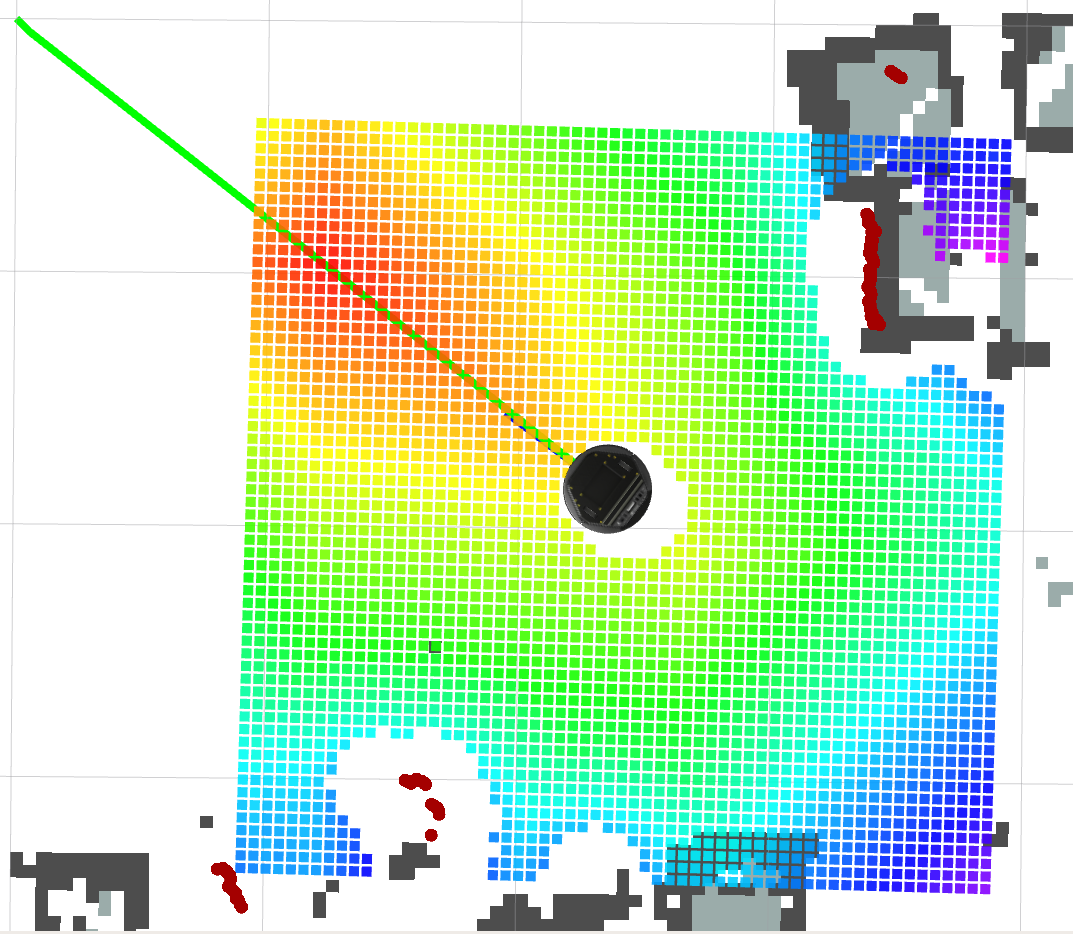
\includegraphics[height=5cm,width=\linewidth]{imgs/chapter5/scan1.png}
        %\caption{Fixed-wing drone (from \cite{parking}).}
        \subcaption{LRF unable to detect the chair, even at close distances}
    \end{minipage}
    \begin{minipage}[b]{.32\linewidth}
        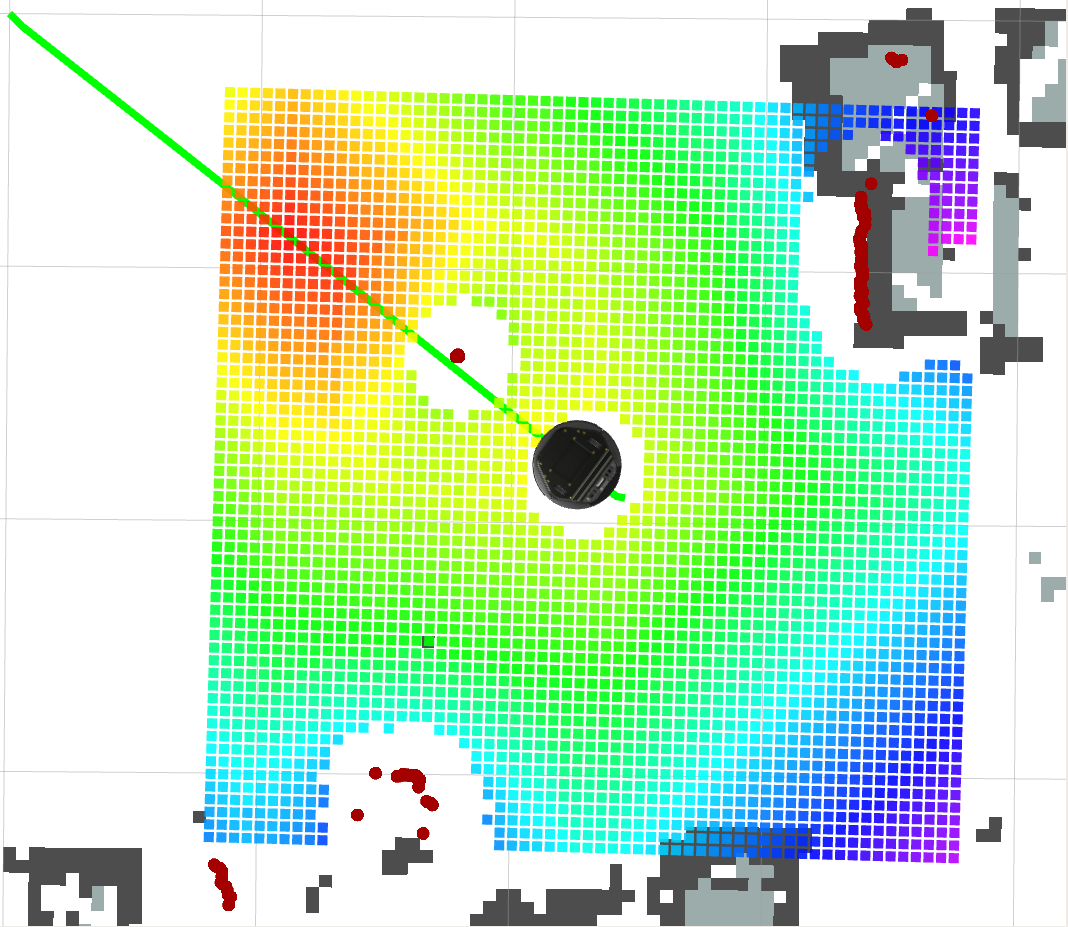
\includegraphics[height=5cm,width=\linewidth]{imgs/chapter5/scan2.png}
        \subcaption{Chair is detected but the plan is still not updated}
        %\caption{Single-rotor drone (from \cite{tumor}).}
    \end{minipage}
     \begin{minipage}[b]{.32\linewidth}
        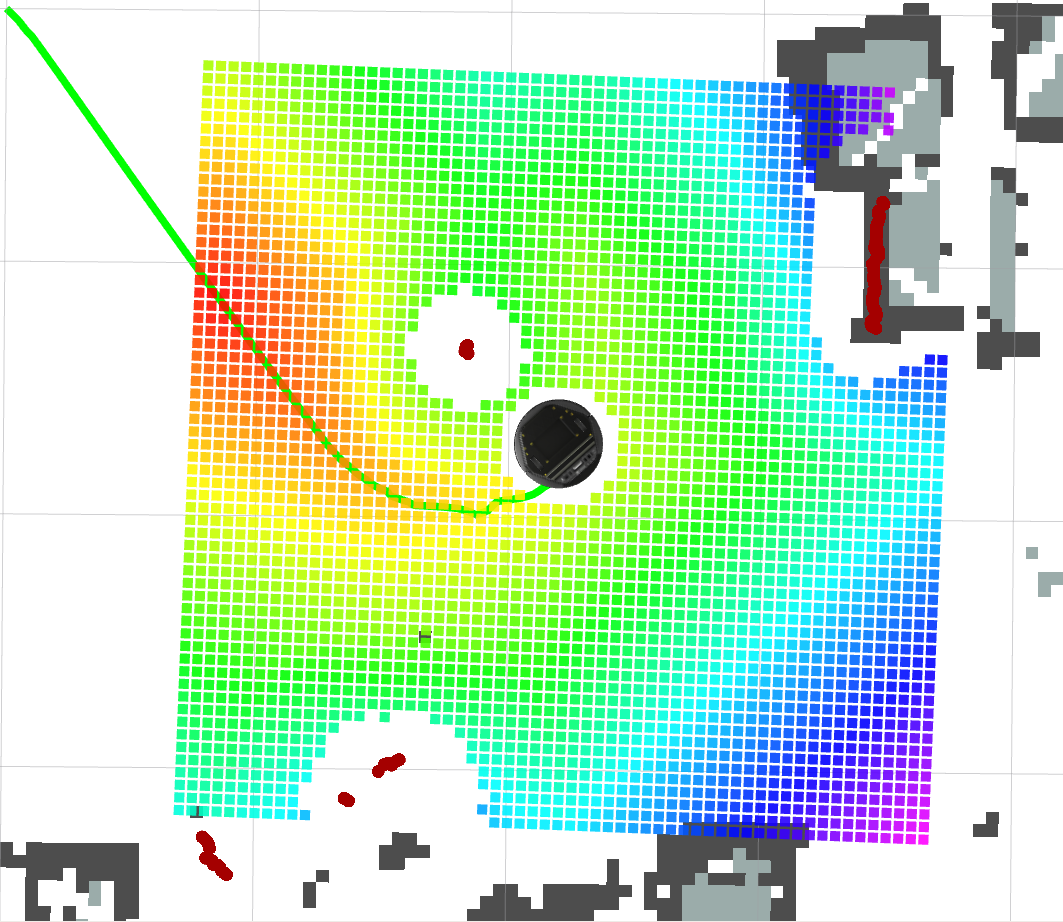
\includegraphics[height=5cm,width=\linewidth]{imgs/chapter5/scan3.png}
        \subcaption{Late replanning after the collision already took place}
    \end{minipage}
    \caption{Navigation results displayed in rviz using the \ac{LRF} as a sensor source}
    \label{fig:scan_results_chair}
\end{figure}
\subsubsection{Radar}
In the radar's case the chair is detected almost immediately, this lead to the global plan and the motion controller to be able to adjust in a very comfortable way in all 5 experiments. Figure X shows some instances of the first experiment. Although the detected space that the chair is occupying has some mismatch, the early detection makes up for it. However since the radar data is inconsistent throughout its frames this may lead to the robot planning a mismatch on paths computed and ultimately lead to some oscillation. ( This can be reduced by using an observation buffer in the radar data. This buffer merges all radar data within a given window of time. However this approach leads to poor performance in very cluttered environments).
\begin{figure}[h] 
    \begin{minipage}[t]{.32\linewidth}
        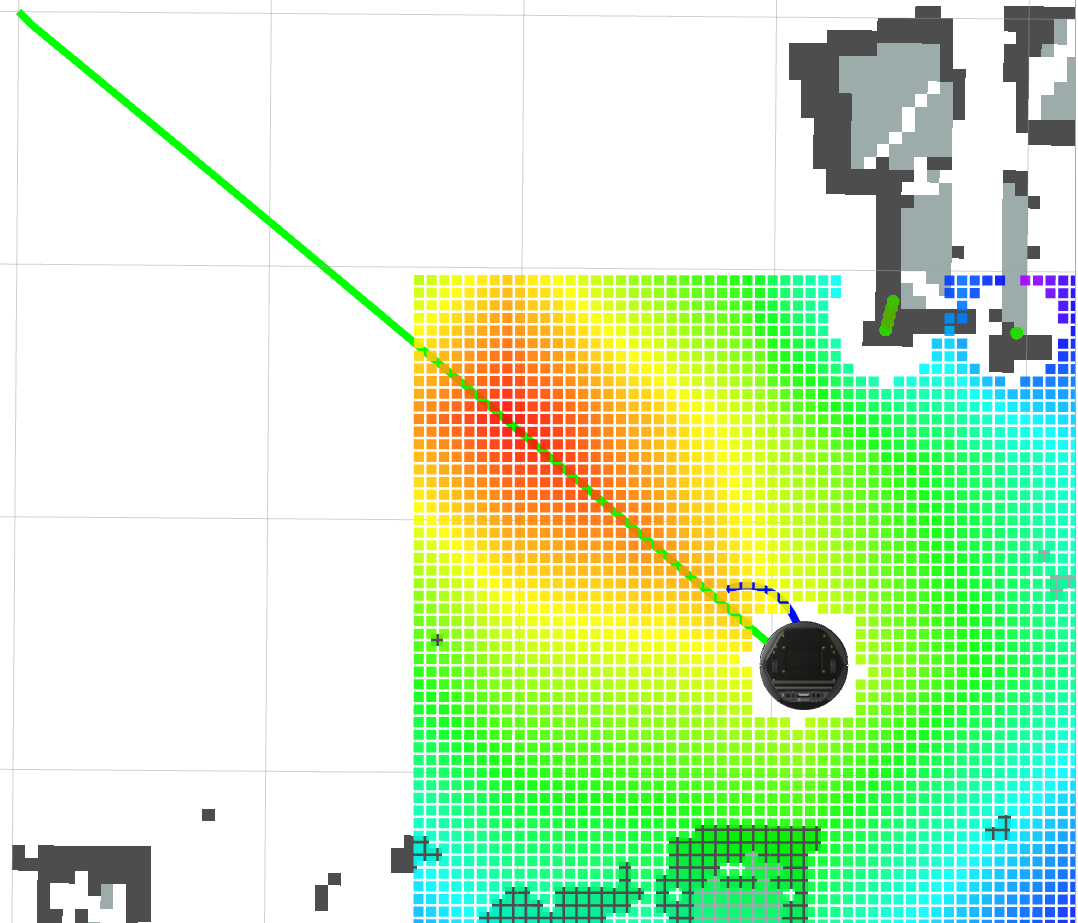
\includegraphics[height=5cm,width=\linewidth]{imgs/chapter5/radar1.png}
        %\caption{Fixed-wing drone (from \cite{parking}).}
        \subcaption{First computed path is a straight line to the goal without not taking into account the obstacle}
    \end{minipage}
    \begin{minipage}[t]{.32\linewidth}
        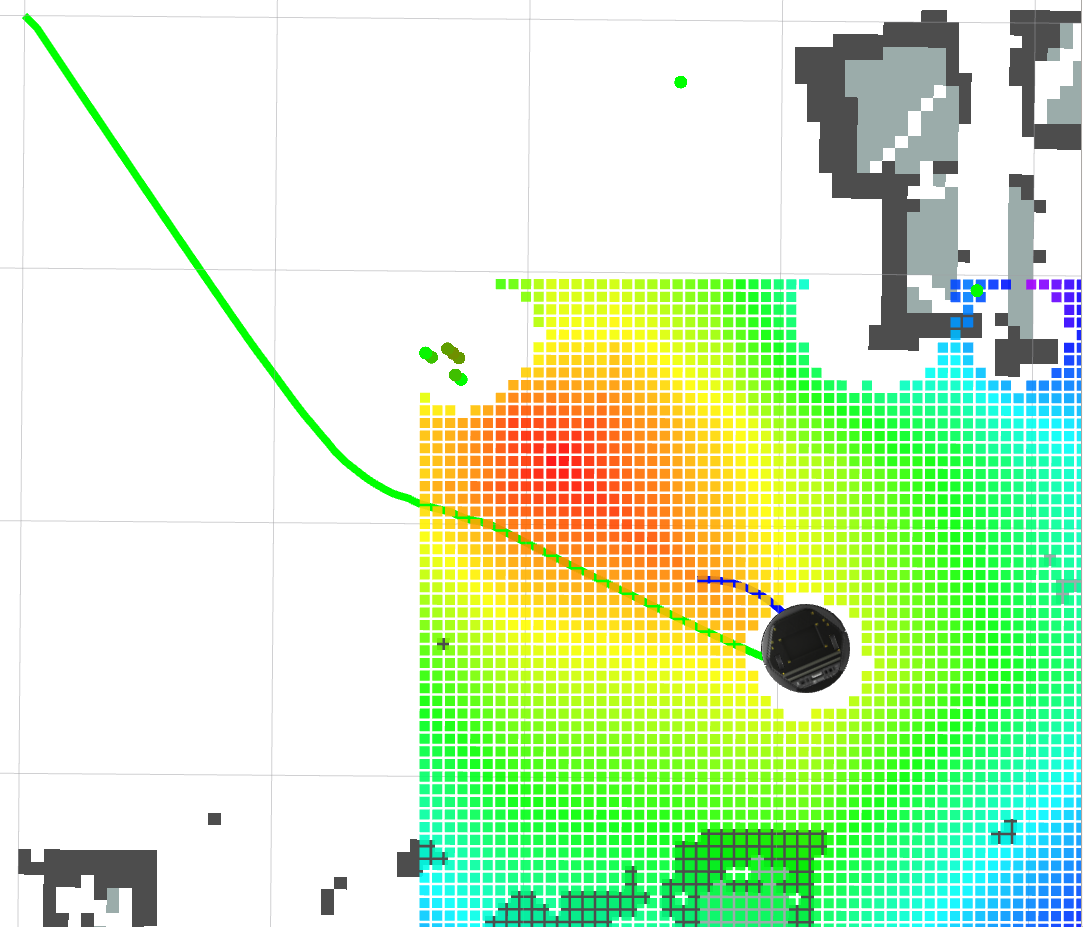
\includegraphics[height=5cm,width=\linewidth]{imgs/chapter5/radar2.png}
        \subcaption{Replanning is done way before collision can occur}
        %\caption{Single-rotor drone (from \cite{tumor}).}
    \end{minipage}
     \begin{minipage}[t]{.32\linewidth}
        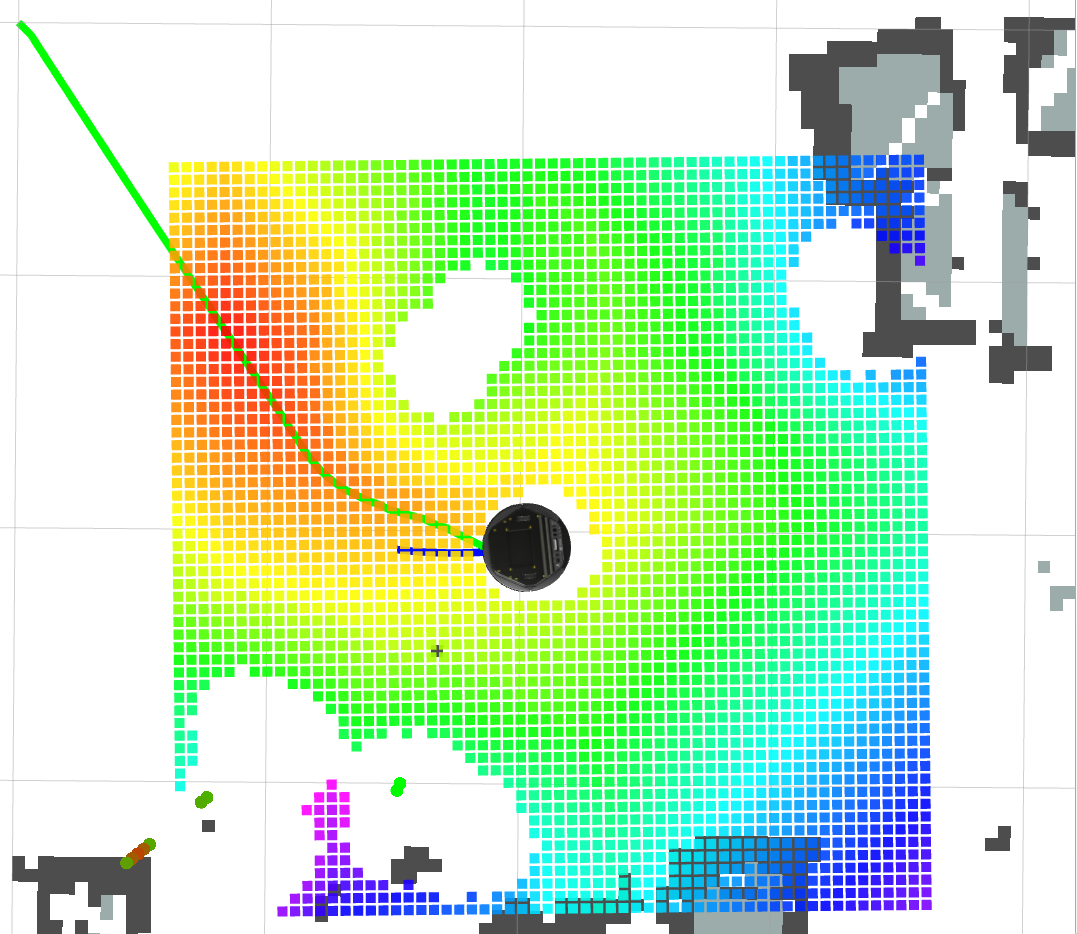
\includegraphics[height=5cm,width=\linewidth]{imgs/chapter5/radar3.png}
        \subcaption{\ac{RADAR} not detecting the chair but it is still marked on the local and global costmap}
    \end{minipage}
    \caption{Navigation results displayed in rviz using the \ac{RADAR} as a sensor source}
    \label{fig:scan_results_chair}
\end{figure}
\subsubsection{Radar and Scan}
Using both sensors showed similar results to the ones shown with only using the radar, the robot was able to avoid the chair all 5 times. 
\section {Experiment 2}
In this following test we wanted to demonstrate two things: (1) the radar detects and avoids persons that obstruct its pre planned path, and (2) if is able to clear previously obstructed spaces (by the person in this case) by raytracing its enviornment. 
\subsection{Setup}
The robot starting position and goal were set the same as the last test, however in this case a single person was instructed to actively obstruct the robot's forward movement until the robot reaches its first goal. After reaching it the person is removed from the environment  and the robot is then instantaneously given a second goal which in this case is the starting position.
\subsection{Results}
\subsection{Laser}
As expected the robot was able to detect and avoid the person in all 5 cases. However it should be noted that in one of this cases the robot tried to avoid it by going through an obstructed space due to a missed detection. This lead to collision. The robot was also able to clear the previously obstructed spaces, getting to the starting position without avoiding past marked obstacles.
\subsection{Radar}
The radar was also able to detect the obstructing person and managed to plan around it in all cases. Since the radar cloud is less dense clearing marked obstacles was slower than in the \ac{LRF} case. However this did not impact the overall performance of the navigation task in a significant way.
\section{Summary}
From this tests we conclude that the \ac{FMCW} radar may be faster at detecting certain indoor obstacles such as chairs which may be crucial when navigating. The radar was also able to perform 
obstacle avoidance of dynamic obstacles(in this case a person that continuously obstructed its path at 5 different times in the same environment which may suggest the use of \ac{RADAR} as an alternate sensory unit over the \ac{LiDAR}.